\begin{frame}[allowframebreaks]{Object Detection with Transformers: DETR}
    \begin{itemize}
        \item DETR (DEtection TRansformer, Carion et al., 2020) introduces a simple and unified object detection pipeline using Transformers.
        \item Transformers replace region proposal networks (RPNs) with attention-based object queries for end-to-end detection.
        \item DETR directly predicts a fixed set of bounding boxes and class labels, eliminating the need for anchors, hand-crafted box proposals, or non-maximum suppression (NMS).
        \item The approach simplifies the pipeline and enables global reasoning, though it may struggle with small objects and require higher compute.
        \item DETR uses bipartite matching (Hungarian algorithm) to uniquely match predicted boxes to ground truth boxes, and is trained end-to-end to regress box coordinates and classify objects.
    \end{itemize}

    \framebreak

    \begin{figure}
        \centering
        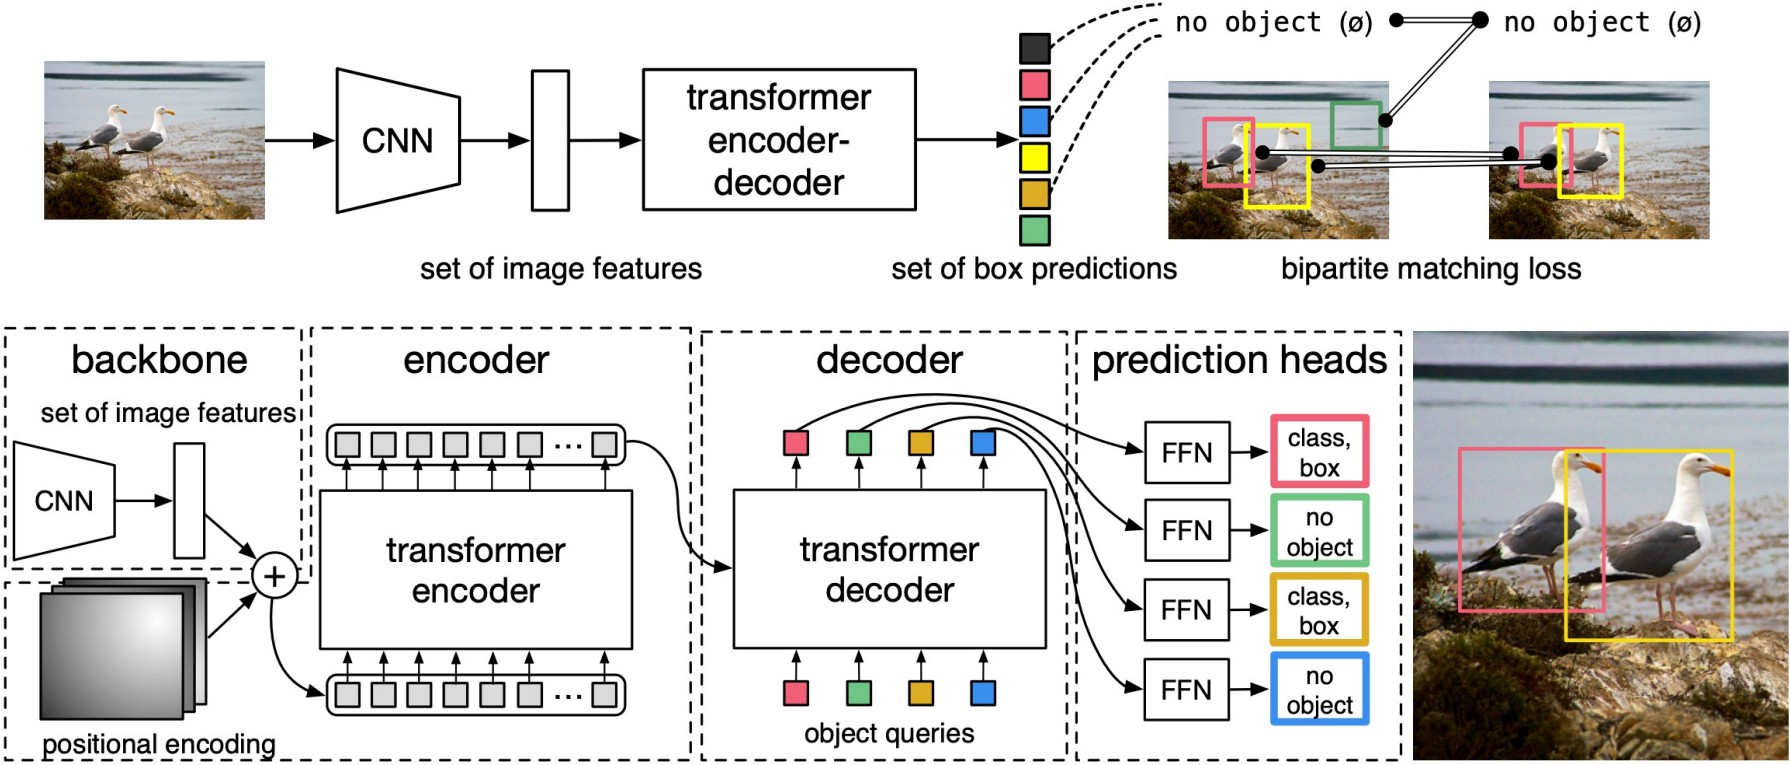
\includegraphics[width=\linewidth,height=0.9\textheight,keepaspectratio]{images/vit/slide_73_1_img.jpg}
        \footnote{Carion et al., “End-to-End Object Detection with Transformers”, ECCV 2020 \url{https://arxiv.org/abs/2005.12872}}
        \footnote{\url{https://docs.google.com/presentation/d/1X0BDhpJOa3IOf29DU8vAB4WJruyLugIX/edit?slide=id.p1#slide=id.p1}}
    \end{figure}
\end{frame}